\section{Recorded run}

This section is generated from saved experiment outputs.

This run uses the complete official training and test splits, with a stratified validation holdout from the training data.

The random seed is 42. The device is \texttt{cpu}. The maximum training budget is 5 epochs per neural configuration, with patience 2. Batch size is 64.

\subsection{imdb results}

Training, validation, and test sizes are 20000, 5000, and 25000, respectively.

\begin{table}[htbp]\centering\small

\caption{Measured performance. Accuracies and macro-F1 are percentages. Time includes neural validation and checkpoint selection.}

\begin{tabular}{lrrrrr}\toprule

Model & Weights & Val.\ acc. & Test acc. & Test F1 & Seconds\\\midrule

baseline & 20,001 & 90.18 & 89.88 & 89.88 & 46.0\\

scratch & 1,322,178 & 81.70 & 80.77 & 80.72 & 147.3\\

\bottomrule\end{tabular}\end{table}

The randomly initialized Transformer changes test accuracy by -9.11 percentage points relative to the TF--IDF baseline. The baseline directly models word and bigram evidence, while the small Transformer learns its embeddings and contextual representation from the task training data. Input truncation and the fixed training budget may also affect the comparison. These possible explanations are not isolated causally by this experiment.

For IMDb, the baseline represents the complete cleaned review, while the Transformer sees only the initial token window. Sentiment evidence later in a review can therefore be unavailable to the Transformer. Its embeddings are learned from task data without language-model pretraining.

For \texttt{scratch}, 73.4\% of training texts exceed the input limit. The selected checkpoint is from epoch 5.

\par\medskip\noindent\begin{minipage}{\linewidth}

\paragraph{Example errors: baseline}

\begin{itemize}

\item True: neg; predicted: pos. "First off let me say, If you haven't enjoyed a Van Damme movie since bloodsport, you probably will not like this movie. Most of these movies may not have the best plots or best act..."

\item True: neg; predicted: pos. "Ben, (Rupert Grint), is a deeply unhappy adolescent, the son of his unhappily married parents. His father, (Nicholas Farrell), is a vicar and his mother, (Laura Linney), is ... wel..."

\end{itemize}

\end{minipage}\par

\par\medskip\noindent\begin{minipage}{\linewidth}

\paragraph{Example errors: scratch}

\begin{itemize}

\item True: neg; predicted: pos. "First off let me say, If you haven't enjoyed a Van Damme movie since bloodsport, you probably will not like this movie. Most of these movies may not have the best plots or best act..."

\item True: neg; predicted: pos. "I had high hopes for this one until they changed the name to 'The Shepherd : Border Patrol, the lamest movie name ever, what was wrong with just 'The Shepherd'. This is a by the nu..."

\end{itemize}

\end{minipage}\par

\begin{figure}[htbp]\centering
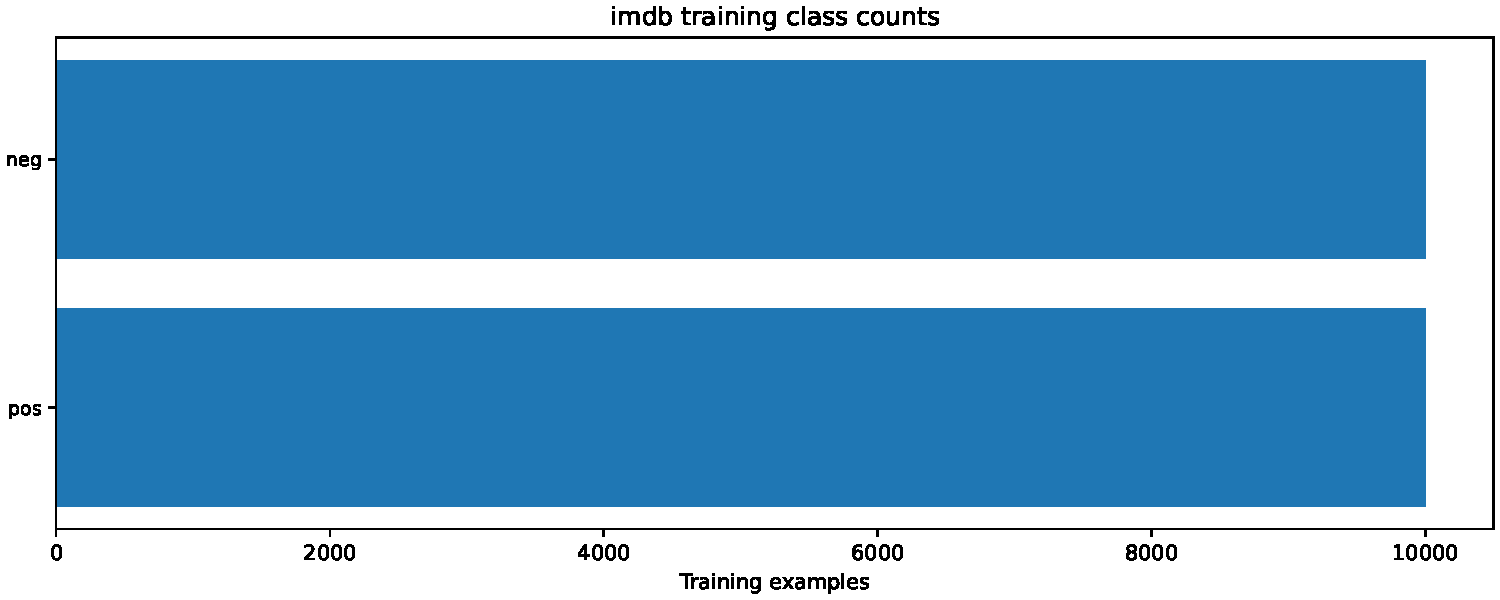
\includegraphics[width=.96\linewidth,height=90mm,keepaspectratio]{output/week5/full/imdb/class_counts.pdf}
\caption{IMDb training class frequencies.}\end{figure}


\begin{figure}[htbp]\centering
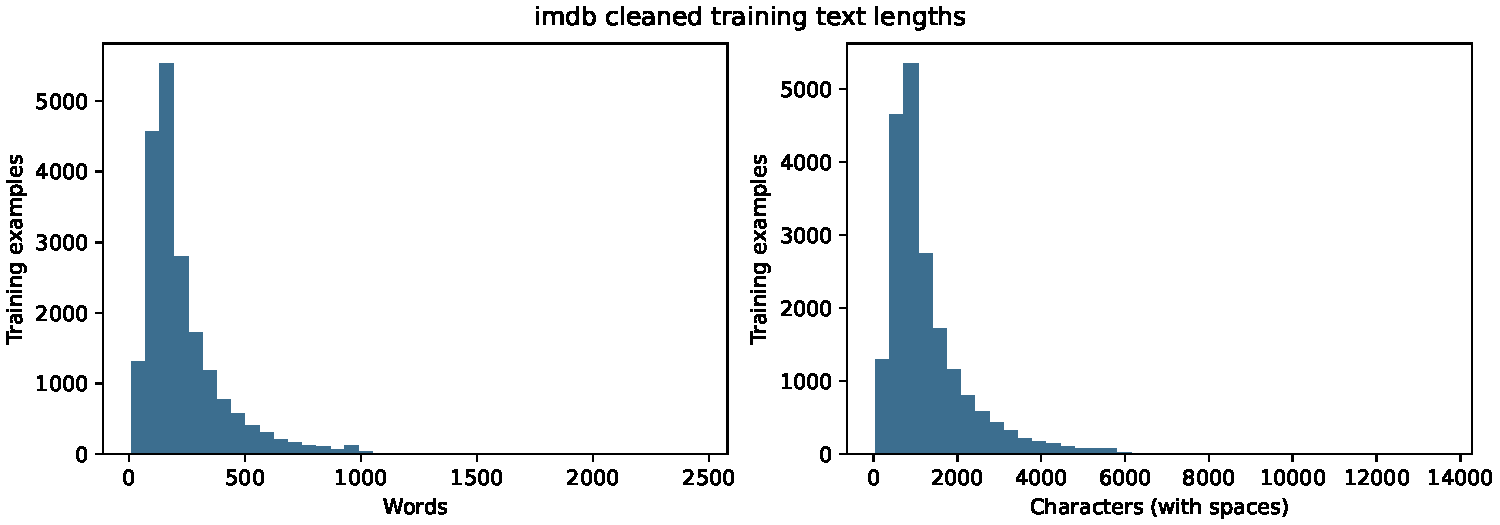
\includegraphics[width=.96\linewidth,height=75mm,keepaspectratio]{output/week5/full/imdb/lengths.pdf}
\caption{imdb cleaned training text lengths.}\end{figure}


\begin{figure}[htbp]\centering
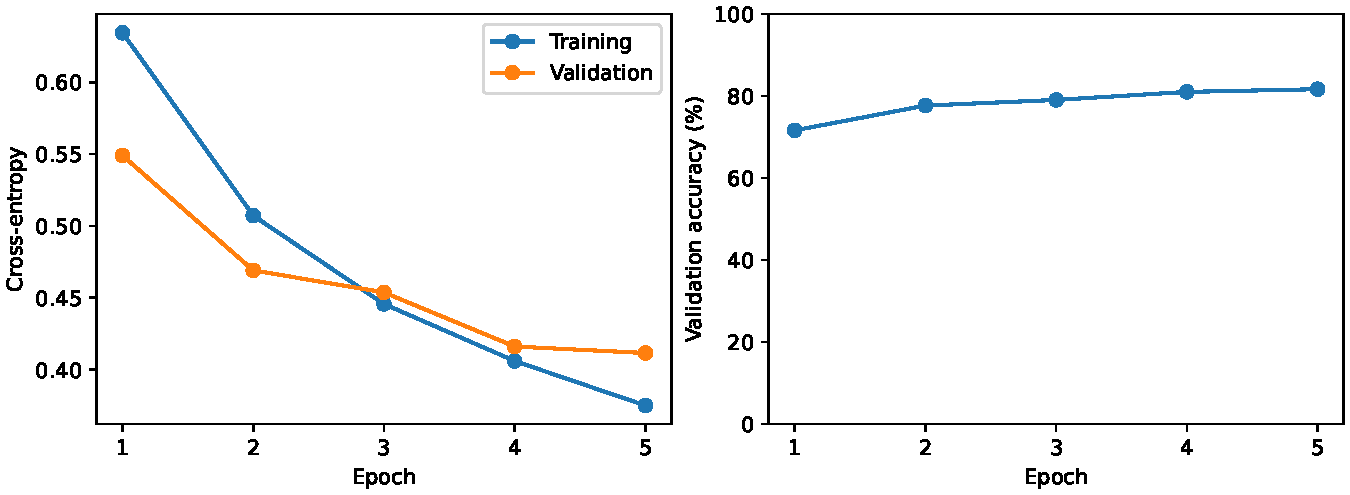
\includegraphics[width=.96\linewidth,height=75mm,keepaspectratio]{output/week5/full/imdb/scratch/learning_curves.pdf}
\caption{imdb randomly initialized Transformer learning curves.}\end{figure}






\clearpage

\subsection{banking77 results}

Training, validation, and test sizes are 8002, 2001, and 3080, respectively.

\begin{table}[htbp]\centering\small

\caption{Measured performance. Accuracies and macro-F1 are percentages. Time includes neural validation and checkpoint selection.}

\begin{tabular}{lrrrrr}\toprule

Model & Weights & Val.\ acc. & Test acc. & Test F1 & Seconds\\\midrule

baseline & 683,991 & 84.71 & 85.49 & 85.39 & 3.6\\

scratch & 139,149 & 51.17 & 49.06 & 46.06 & 17.5\\

transfer\_full & 4,395,853 & 84.01 & 83.12 & 82.40 & 83.2\\

transfer\_head & 9,933 & 15.34 & 13.02 & 9.38 & 22.1\\

transfer\_lower & 208,205 & 70.46 & 70.58 & 68.89 & 60.8\\

transfer\_upper & 208,205 & 72.26 & 69.90 & 68.55 & 51.8\\

\bottomrule\end{tabular}\end{table}

The randomly initialized Transformer changes test accuracy by -36.43 percentage points relative to the TF--IDF baseline. The baseline directly models word and bigram evidence, while the small Transformer learns its embeddings and contextual representation from the task training data. Input truncation and the fixed training budget may also affect the comparison. These possible explanations are not isolated causally by this experiment.

BANKING77 has 77 classes and only 103.9 training queries per class on average. Short domain-specific queries can provide useful word and bigram cues to the baseline, while the random Transformer must learn representations and a 77-way decision rule within the fixed epoch budget. The recorded truncation fractions help distinguish input-length effects from these factors.

The validation-selected fine-tuning configuration is \texttt{transfer\_full}, with test accuracy 83.12\%. Selection uses validation accuracy; test results are reported afterward.

The measured validation Pareto frontier contains transfer\_full, transfer\_head, transfer\_upper.

Full fine-tuning changes test accuracy by +70.10 percentage points relative to head-only training. The upper- and lower-block runs each unfreeze one encoder block, enabling a comparison at the same block budget.

Unfreezing the upper block changes validation accuracy by +1.80 percentage points relative to unfreezing the lower block. The corresponding test difference is -0.68 percentage points. This quantifies layer-position sensitivity for this checkpoint and training budget.

The fully fine-tuned pretrained model changes test accuracy by +34.06 percentage points relative to the random Transformer. Pretraining and architecture both differ in this comparison, so their effects are not isolated.

For \texttt{scratch}, 0.0\% of training texts exceed the input limit. The selected checkpoint is from epoch 5.

For \texttt{transfer\_full}, 0.0\% of training texts exceed the input limit. The selected checkpoint is from epoch 5.

For \texttt{transfer\_head}, 0.0\% of training texts exceed the input limit. The selected checkpoint is from epoch 5.

For \texttt{transfer\_lower}, 0.0\% of training texts exceed the input limit. The selected checkpoint is from epoch 5.

For \texttt{transfer\_upper}, 0.0\% of training texts exceed the input limit. The selected checkpoint is from epoch 5.

\par\medskip\noindent\begin{minipage}{\linewidth}

\paragraph{Example errors: baseline}

\begin{itemize}

\item True: card\_arrival; predicted: card\_linking. "How do I locate my card?..."

\item True: card\_arrival; predicted: transfer\_not\_received\_by\_recipient. "I ordered a card but it has not arrived. Help please!..."

\end{itemize}

\end{minipage}\par

\par\medskip\noindent\begin{minipage}{\linewidth}

\paragraph{Example errors: scratch}

\begin{itemize}

\item True: card\_arrival; predicted: card\_linking. "How do I locate my card?..."

\item True: card\_arrival; predicted: card\_not\_working. "I ordered a card but it has not arrived. Help please!..."

\end{itemize}

\end{minipage}\par

\par\medskip\noindent\begin{minipage}{\linewidth}

\paragraph{Example errors: transfer\_full}

\begin{itemize}

\item True: card\_arrival; predicted: card\_delivery\_estimate. "Is there a way to know when my card will arrive?..."

\item True: card\_arrival; predicted: card\_delivery\_estimate. "When will I get my card?..."

\end{itemize}

\end{minipage}\par

\par\medskip\noindent\begin{minipage}{\linewidth}

\paragraph{Example errors: transfer\_head}

\begin{itemize}

\item True: card\_arrival; predicted: verify\_top\_up. "How do I locate my card?..."

\item True: card\_arrival; predicted: wrong\_amount\_of\_cash\_received. "I still have not received my new card, I ordered over a week ago...."

\end{itemize}

\end{minipage}\par

\par\medskip\noindent\begin{minipage}{\linewidth}

\paragraph{Example errors: transfer\_lower}

\begin{itemize}

\item True: card\_arrival; predicted: card\_linking. "How do I locate my card?..."

\item True: card\_arrival; predicted: card\_delivery\_estimate. "Is there a way to know when my card will arrive?..."

\end{itemize}

\end{minipage}\par

\par\medskip\noindent\begin{minipage}{\linewidth}

\paragraph{Example errors: transfer\_upper}

\begin{itemize}

\item True: card\_arrival; predicted: lost\_or\_stolen\_card. "How do I locate my card?..."

\item True: card\_arrival; predicted: card\_delivery\_estimate. "Is there a way to know when my card will arrive?..."

\end{itemize}

\end{minipage}\par

\begin{figure}[htbp]\centering
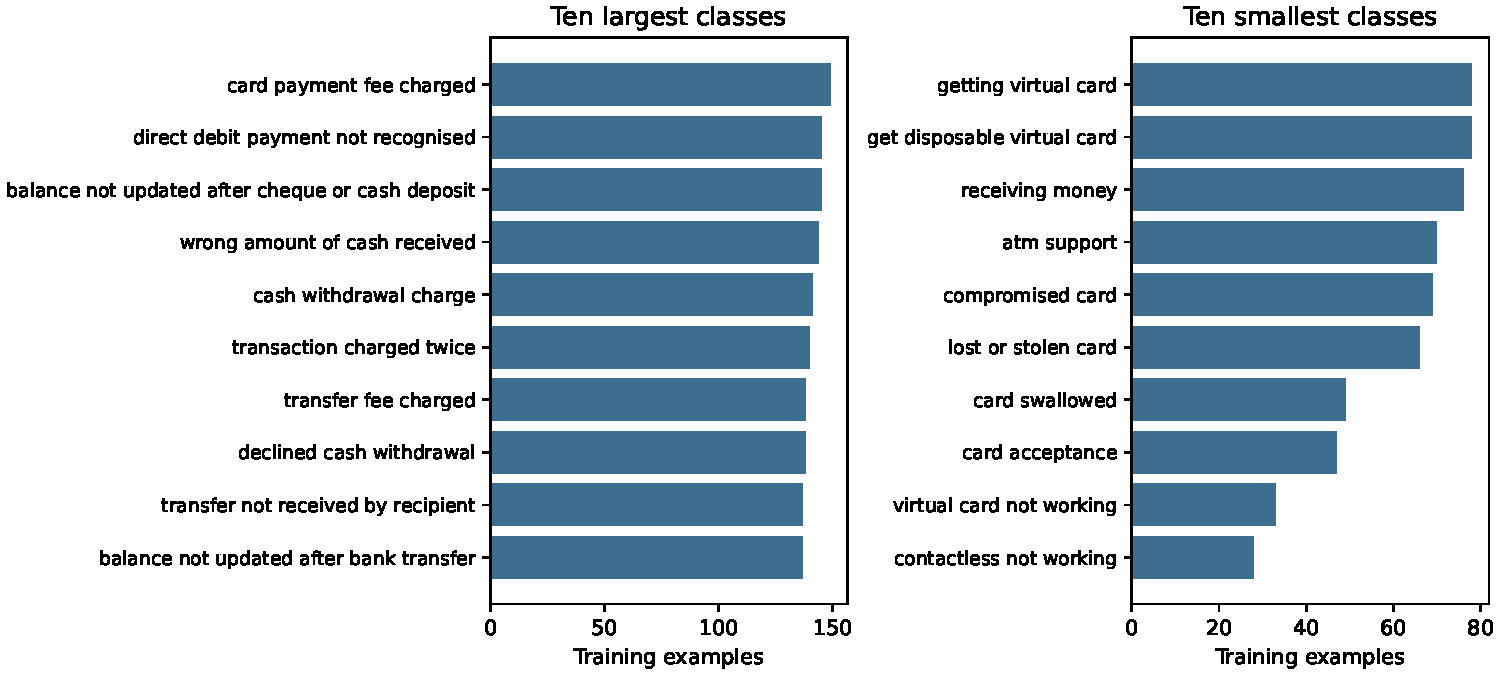
\includegraphics[width=.96\linewidth,height=90mm,keepaspectratio]{output/week5/full/banking77/class_overview.pdf}
\caption{BANKING77 ten largest and ten smallest training classes. The complete 77-class plot is saved separately as class\_counts.pdf.}\end{figure}


\begin{figure}[htbp]\centering
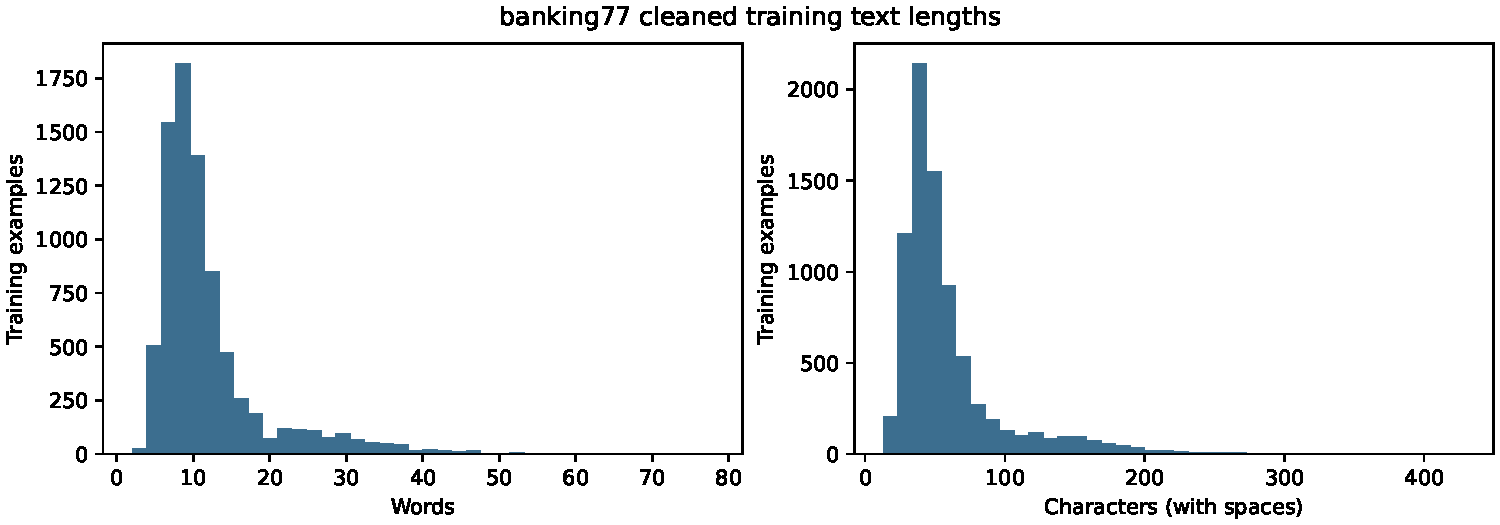
\includegraphics[width=.96\linewidth,height=75mm,keepaspectratio]{output/week5/full/banking77/lengths.pdf}
\caption{banking77 cleaned training text lengths.}\end{figure}


\begin{figure}[htbp]\centering
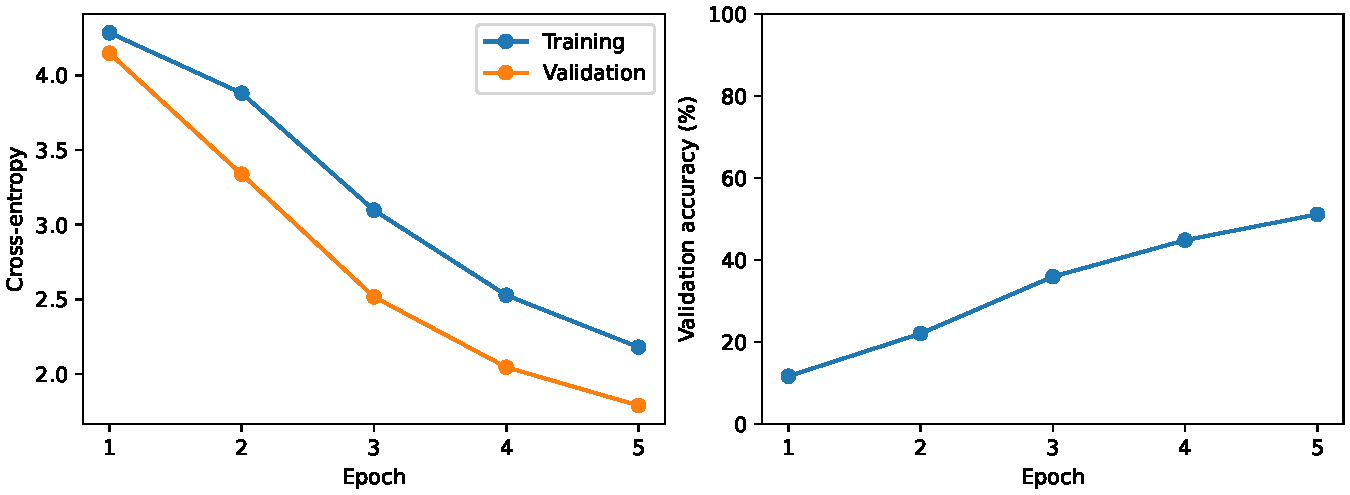
\includegraphics[width=.96\linewidth,height=75mm,keepaspectratio]{output/week5/full/banking77/scratch/learning_curves.pdf}
\caption{banking77 randomly initialized Transformer learning curves.}\end{figure}


\begin{figure}[htbp]\centering
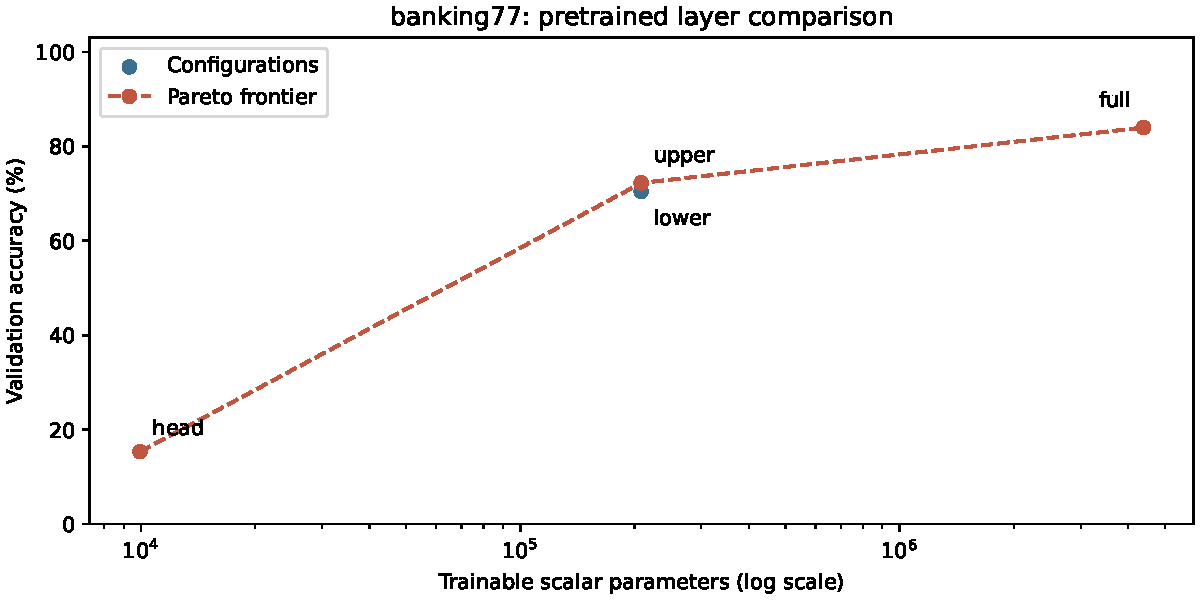
\includegraphics[width=.96\linewidth,height=75mm,keepaspectratio]{output/week5/full/banking77/pareto_validation.pdf}
\caption{banking77 validation Pareto frontier used for configuration comparison.}\end{figure}


\begin{figure}[htbp]\centering
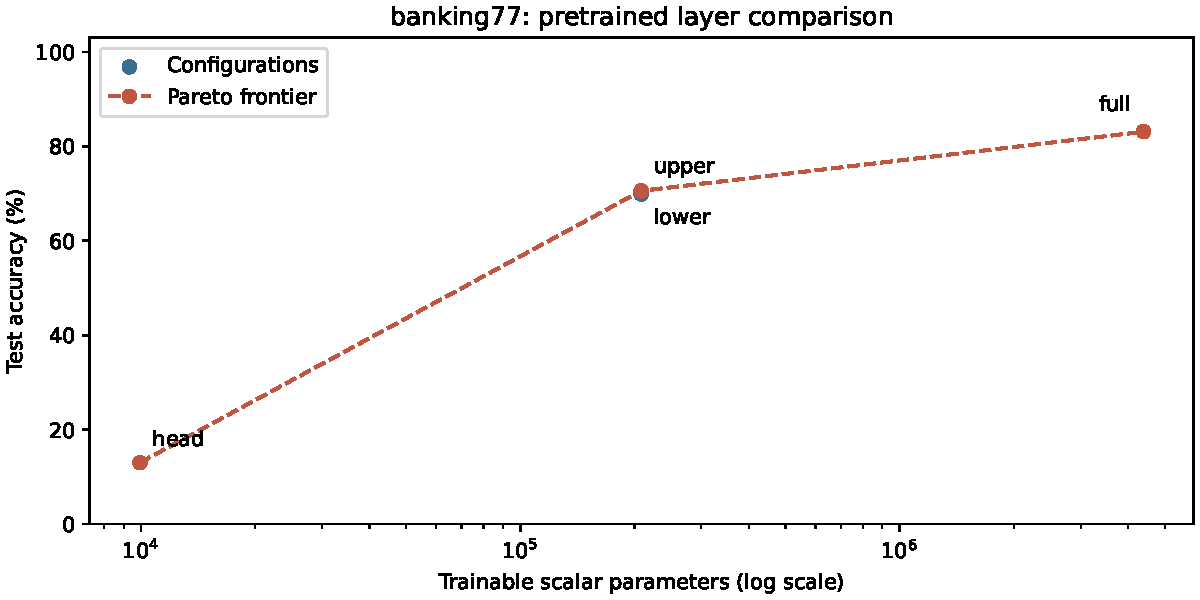
\includegraphics[width=.96\linewidth,height=75mm,keepaspectratio]{output/week5/full/banking77/pareto_test.pdf}
\caption{banking77 test accuracy versus trained weights; descriptive evaluation.}\end{figure}


\clearpage

\section{Conclusions and limitations}

Results use one random seed, one fixed hyperparameter budget, and a compact pretrained BERT checkpoint. Accuracy differences do not establish that one architecture is universally better. Broader learning-rate searches, repeated seeds, and larger checkpoints could change the ranking. Fine-tuning importance is assessed through the tested frozen-layer configurations.

For imdb, the highest validation accuracy among completed models is obtained by \texttt{baseline}. Its held-out test accuracy is 89.88\%.

For banking77, the highest validation accuracy among completed models is obtained by \texttt{baseline}. Its held-out test accuracy is 85.49\%.